% Native editable composition from verified, unchanged IDE images.
\begin{figure}[htbp]
\centering
\sbox0{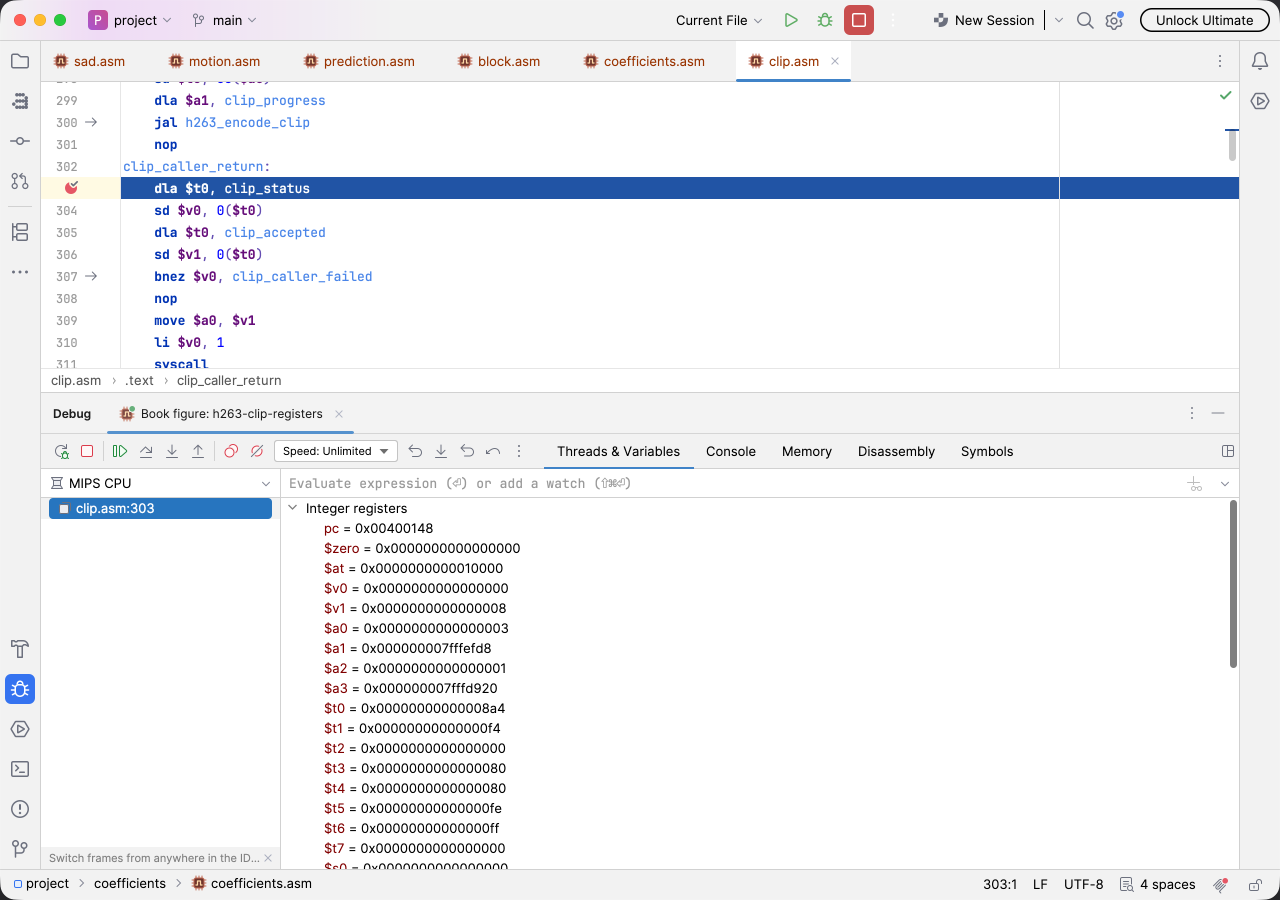
\includegraphics[artifact]{book/captures/035-h263/h263-clip-accepted/registers.png}}
\sbox2{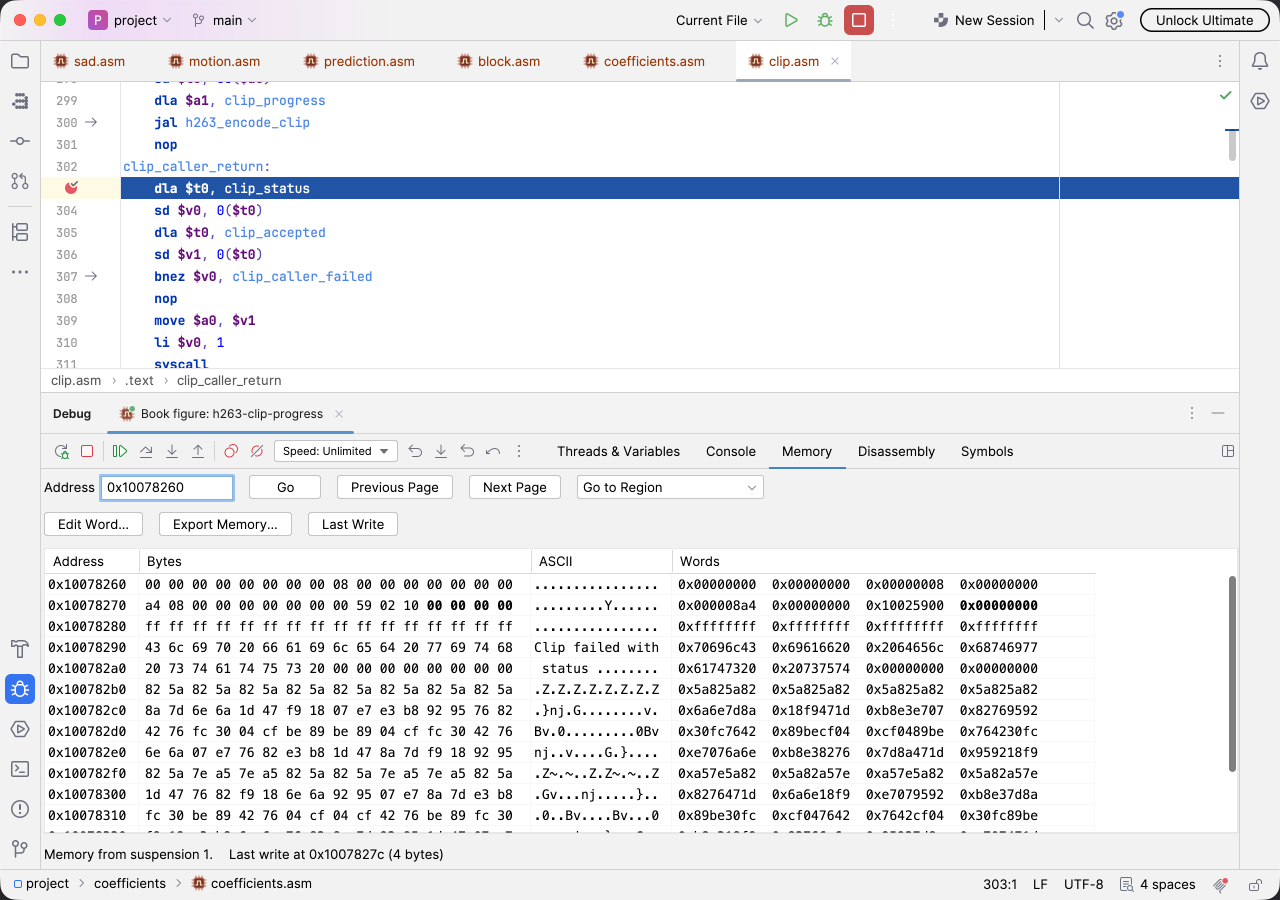
\includegraphics[artifact]{book/captures/035-h263/h263-clip-accepted/progress.png}}
\edef\MARSclipsourceLeft{\the\dimexpr0.036718750\wd0\relax}
\edef\MARSclipsourceBottom{\the\dimexpr0.774444444\ht0\relax}
\edef\MARSclipsourceRight{\the\dimexpr0.611718750\wd0\relax}
\edef\MARSclipsourceTop{\the\dimexpr0.170000000\ht0\relax}
\edef\MARSclipprogressLeft{\the\dimexpr0.520312500\wd2\relax}
\edef\MARSclipprogressBottom{\the\dimexpr0.312222222\ht2\relax}
\edef\MARSclipprogressRight{\the\dimexpr0.139843750\wd2\relax}
\edef\MARSclipprogressTop{\the\dimexpr0.634444444\ht2\relax}
\edef\MARSclipreturnsLeft{\the\dimexpr0.246093750\wd0\relax}
\edef\MARSclipreturnsBottom{\the\dimexpr0.310000000\ht0\relax}
\edef\MARSclipreturnsRight{\the\dimexpr0.596875000\wd0\relax}
\edef\MARSclipreturnsTop{\the\dimexpr0.638888889\ht0\relax}
\begin{tikzpicture}[alt={Three annotated details at clip_caller_return. Register v0 is zero and v1 is eight. The Words view begins with a doubleword before the progress record. The next low/high pairs contain accepted count eight, encoded-byte count 8a4 or 2212 and final reference pointer 10025900. The highlighted dla precedes the caller status store.}]
\node[anchor=north west,inner sep=0,font=\small\bfseries] (source-title) at (6mm,0) {The whole clip call has returned};
\node[anchor=north west,inner sep=0] (source) at ([yshift=-1mm]source-title.south west) {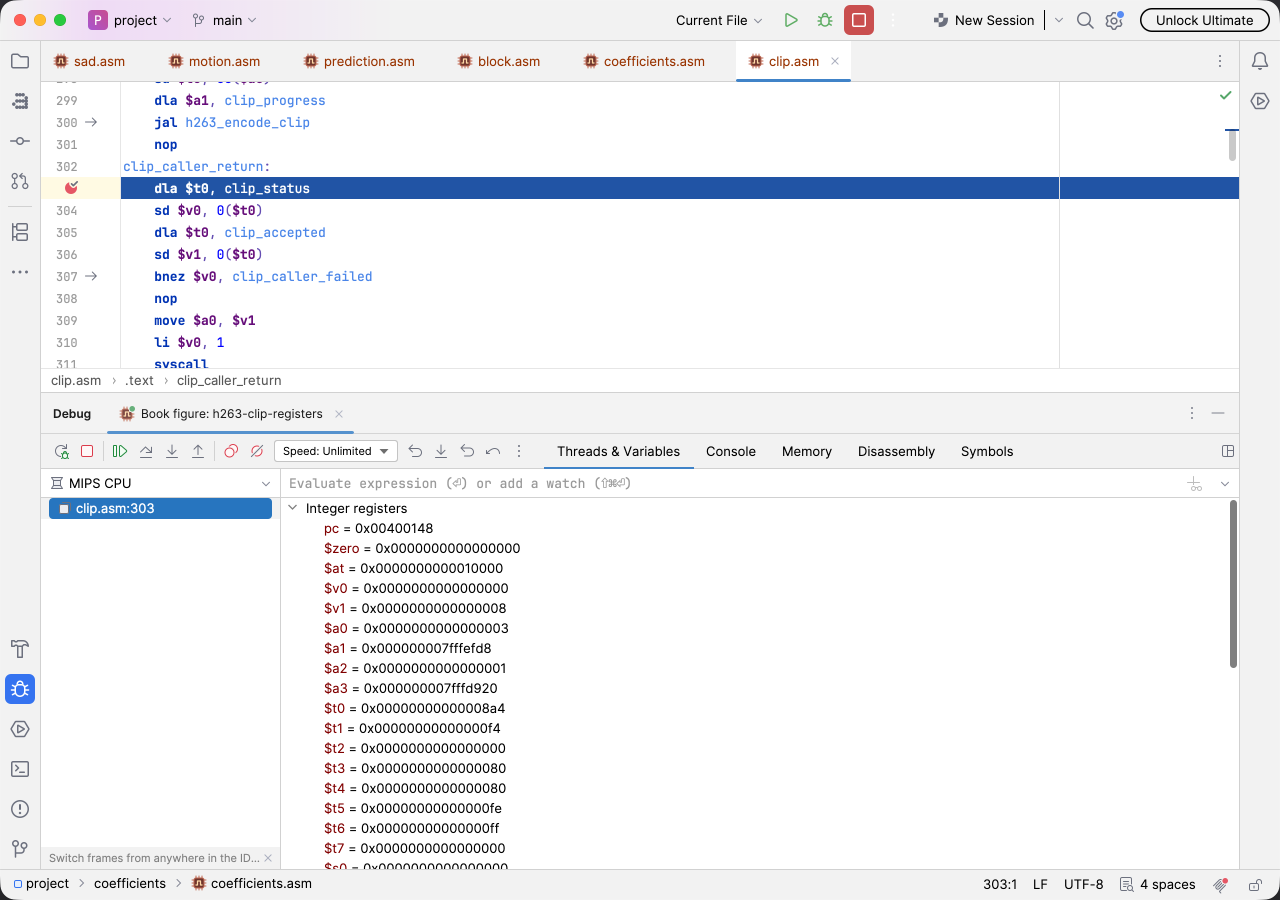
\includegraphics[width=0.7\linewidth,artifact,trim={\MARSclipsourceLeft{} \MARSclipsourceBottom{} \MARSclipsourceRight{} \MARSclipsourceTop{}},clip]{book/captures/035-h263/h263-clip-accepted/registers.png}};
\begin{scope}[shift={(source.south west)},x={($(source.south east)-(source.south west)$)},y={($(source.north west)-(source.south west)$)}]
\draw[black,line width=0.7pt] (0.168888889,0.080000000) rectangle (0.584444444,0.520000000);
\node[draw=black,fill=white,circle,inner sep=1.5pt,font=\footnotesize] at ($(0.168888889,0.520000000)+(-3mm,0)$) {1};
\end{scope}
\node[anchor=north west,inner sep=0,font=\small\bfseries] (progress-title) at ([yshift=-2mm]source.south west) {Accepted count, encoded bytes and reference pointer};
\node[anchor=north west,inner sep=0] (progress) at ([yshift=-1mm]progress-title.south west) {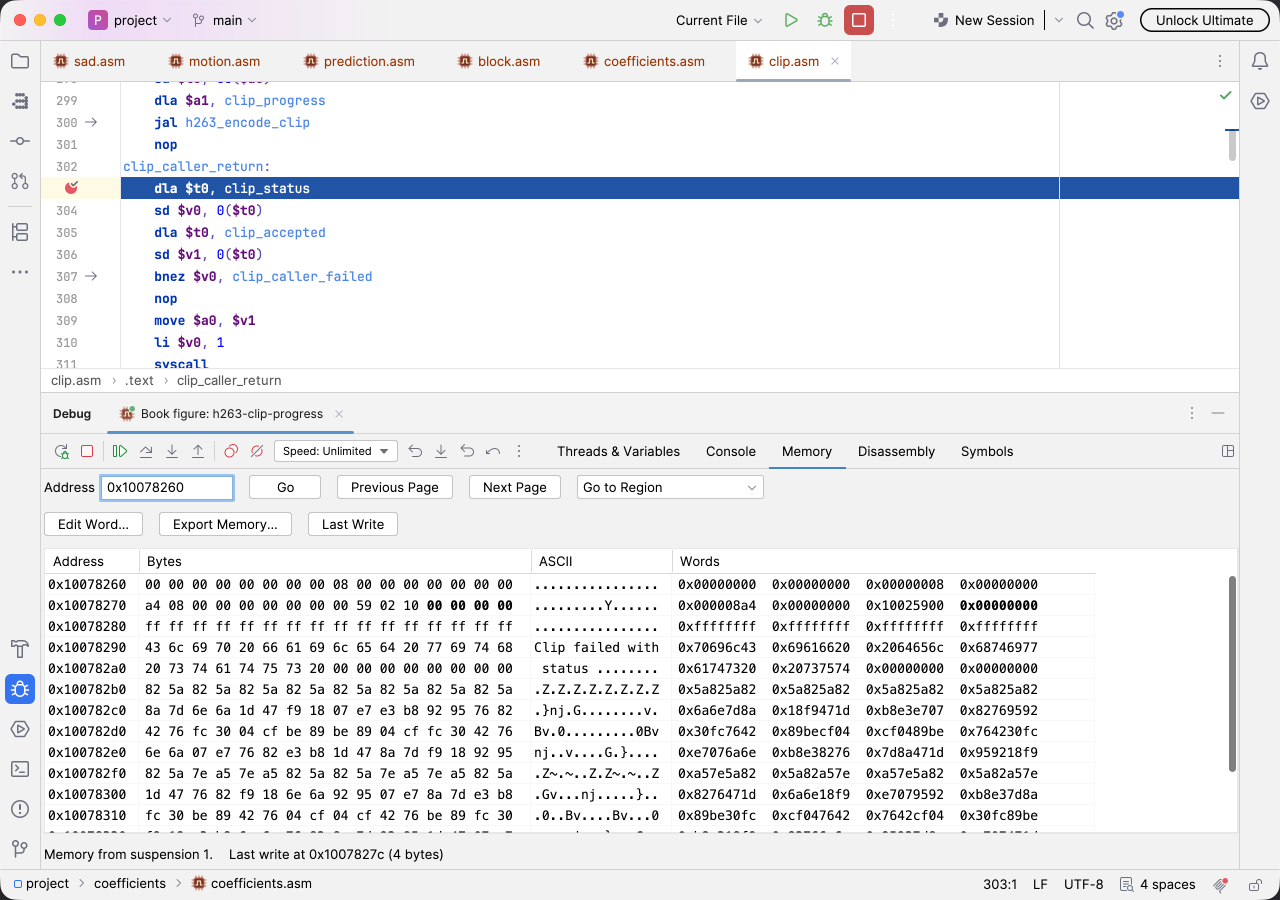
\includegraphics[width=0.84\linewidth,artifact,trim={\MARSclipprogressLeft{} \MARSclipprogressBottom{} \MARSclipprogressRight{} \MARSclipprogressTop{}},clip]{book/captures/035-h263/h263-clip-accepted/progress.png}};
\begin{scope}[shift={(progress.south west)},x={($(progress.south east)-(progress.south west)$)},y={($(progress.north west)-(progress.south west)$)}]
\draw[black,line width=0.7pt] (0.013793103,0.062500000) rectangle (0.986206897,0.937500000);
\node[draw=black,fill=white,circle,inner sep=1.5pt,font=\footnotesize] at ($(0.013793103,0.937500000)+(-3mm,0)$) {2};
\end{scope}
\node[anchor=north west,inner sep=0,font=\small\bfseries] (returns-title) at ([yshift=-2mm]progress.south west) {Whole-clip status and accepted-picture count};
\node[anchor=north west,inner sep=0] (returns) at ([yshift=-1mm]returns-title.south west) {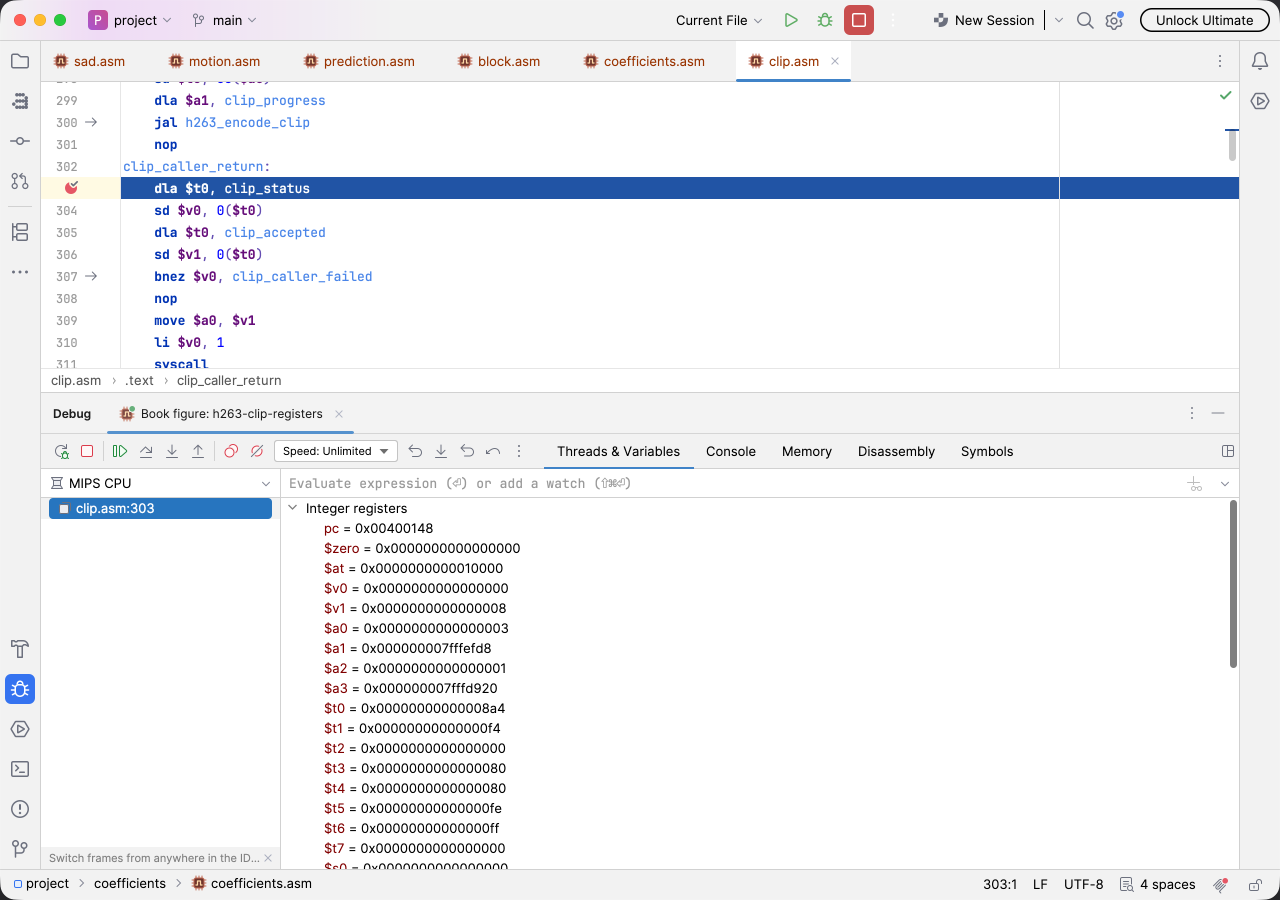
\includegraphics[width=0.5\linewidth,artifact,trim={\MARSclipreturnsLeft{} \MARSclipreturnsBottom{} \MARSclipreturnsRight{} \MARSclipreturnsTop{}},clip]{book/captures/035-h263/h263-clip-accepted/registers.png}};
\begin{scope}[shift={(returns.south west)},x={($(returns.south east)-(returns.south west)$)},y={($(returns.north west)-(returns.south west)$)}]
\draw[black,line width=0.7pt] (0.029850746,0.065217391) rectangle (0.970149254,0.934782609);
\node[draw=black,fill=white,circle,inner sep=1.5pt,font=\footnotesize] at ($(0.029850746,0.934782609)+(-3mm,0)$) {3};
\end{scope}
\end{tikzpicture}
\par\smallskip
\begin{minipage}{\linewidth}
\small
\begin{enumerate}
\item The input contains eight generated QCIF pictures at approximately five frames per second, lasting 1.6016 seconds. This call has completed required writes, the EOF probe and descriptor cleanup. Independent file checks establish those operations.
\item The first doubleword precedes the progress record. Starting at the third displayed 32-bit word, read low/high pairs across the row boundary: accepted count eight, encoded count \texttt{0x8a4}=2212 bytes and accepted reference pointer \texttt{0x10025900}. The pointer names the last accepted reconstruction, not the raw input buffer.
\item \texttt{\$v0}=0 establishes whole-clip success; \texttt{\$v1}=8 is the accepted count. A nonzero status can retain accepted progress, so the count alone is insufficient. Both outputs written in these IDE runs match the independently decoded oracle byte for byte.
\end{enumerate}
\end{minipage}
\caption{The generated eight-picture clip after all required writes and closes. Two Debug launches inspect the same completed encoder.}
\label{fig:h263-clip-accepted}
\end{figure}
